\documentclass{beamer}
\title[PCR]{A Hands-on Approach to Learning Molecular Biology Techniques}
\subtitle{Team Q}
\author{R.~Barnie \and D.~Jonins \and D.~McElroy \and M.~Ross \and R.~Taylor}
\date{March 19, 2013} 

\usepackage{gensymb}
\begin{document}

\section{Introduction}
\frame{\titlepage}
%INTRO:                                                                                  
%    - what is the project?                                                          DAN
%    - what is pcr and why is it important?
%    - what are primers?
%    - explain "simulation" (DO NOT SAY) to save time and money
%    - explain rules themselves    
\begin{frame}
\frametitle{Project Outline}
\end{frame}    

\begin{frame}
\frametitle{What Is PCR?}
\end{frame}

\begin{frame}
\frametitle{Why Is PCR Important?}
\end{frame}

\begin{frame}
\frametitle{Primers - What Do?}
\end{frame}

\begin{frame}
\frametitle{Primer Rules - 1}

\begin{itemize}
\item Melting temperature within 50 - 65\degree C
\item Unique to the strand
\item Ends in base \texttt{g} or \texttt{c}
\item Bases do not repeat more than 3 times in a row
\item Length between 20 and 30
\item \texttt{gc} content between 40-60\%
\end{itemize}

\end{frame}
     


\section{Group Organisation}
\begin{frame}
\frametitle{Team Roles}

\begin{description}
\item[Ross Barnie]{Toolsmith, Librarian}
\item[Dmitrijs Jonins]{Project Manager}
\item[Daniel McElroy]{Lead Programmer}
\item[Murray Ross]{Quality Assurance Manager, Test Manager}	
\item[Ross Taylor]{Customer Liaison}
\end{description}

\end{frame}

\begin{frame}
\frametitle{Implementation Sub-Teams}

\begin{description}
\item[User Interface]{Ross Barnie, Murray Ross}
\item[Models and Methods]{Daniel McElroy, Ross Taylor}
\item[Animation]{Dmitrijs Jonins}
\end{description}

\end{frame}


\section{Design}
\begin{frame}
\frametitle{Current Systems [1]}

\begin{itemize}
\item http://youtu.be/XXkG6m3yT1M
\item This is a video made by the Biology Department itself.
\item Very short.
\item Very small amount of information.
\item No interactivity.
\item No information about Primer Design.
\end{itemize}
\end{frame}

\begin{frame}
\frametitle{Current Systems [1]}
\begin{figure}
  \begin{center}
    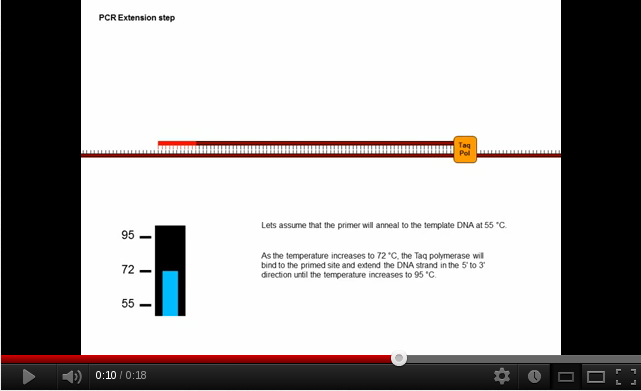
\includegraphics[width=0.8\textwidth]{./img/currentSystems1.png}
  \end{center}
\end{figure}
\end{frame}

\begin{frame}
\frametitle{Current Systems [2]}
\begin{itemize}
\item http://youtu.be/JRAA4C2OPwg
\item Better than System [1] but still not great
\item Longer than [1].
\item More information about PCR process.
\item Again, no interactivity or information about Primer Design
\end{itemize}
\end{frame}

\begin{frame}
\frametitle{Current Systems [2]}
\begin{figure}
  \begin{center}
    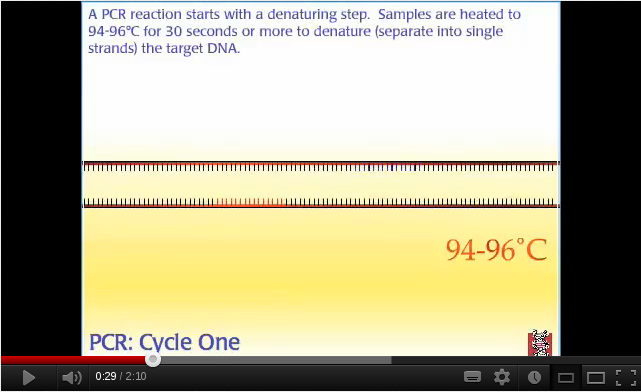
\includegraphics[width=0.8\textwidth]{./img/currentSystems2-1.png}
  \end{center}
\end{figure}
\end{frame}

\begin{frame}
\frametitle{Current Systems [2]}
\begin{figure}
  \begin{center}
    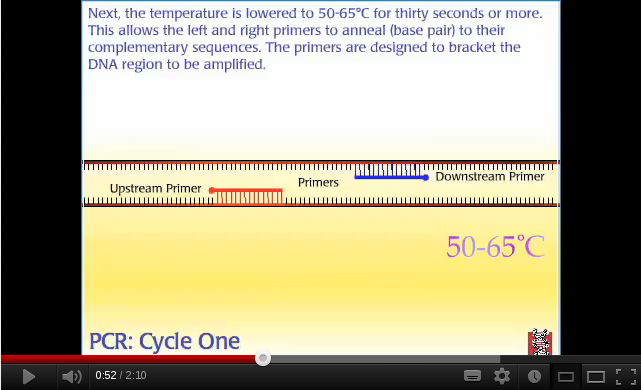
\includegraphics[width=0.8\textwidth]{./img/currentSystems2-2.png}
  \end{center}
\end{figure}
\end{frame}

\begin{frame}
\frametitle{Current Systems [2]}
\begin{figure}
  \begin{center}
    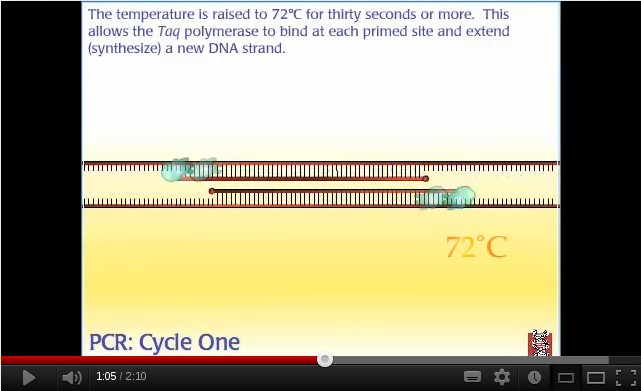
\includegraphics[width=0.8\textwidth]{./img/currentSystems2-3.png}
  \end{center}
\end{figure}
\end{frame}

\begin{frame}
\frametitle{Current Systems [2]}
\begin{figure}
  \begin{center}
    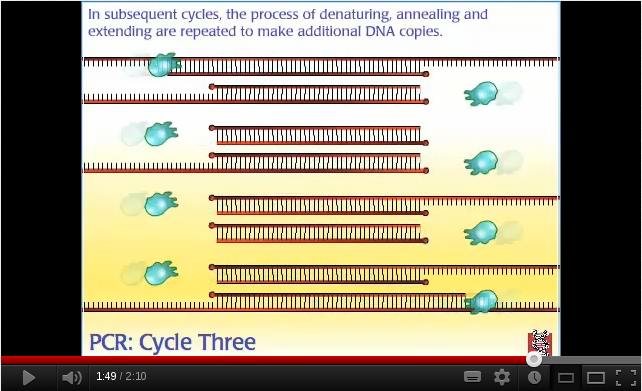
\includegraphics[width=0.8\textwidth]{./img/currentSystems2-4.png}
  \end{center}
\end{figure}
\end{frame}

\begin{frame}
\frametitle{Current Systems [3]}
\begin{itemize}
\item http://learn.genetics.utah.edu/content/labs/pcr/
\item Visually more detailed and impressive
\item Includes a lot of detail about PCR.
\item However, also includes a lot of information about basic biology
which is not necessary for Level 3 students.
\item Has some interactivity but the reason for the actions being
performed is not clear.
\item Again, no focus given to Primer Design.
\end{itemize}
\end{frame}

\begin{frame}
\frametitle{Current Systems [3]}
\begin{figure}
  \begin{center}
    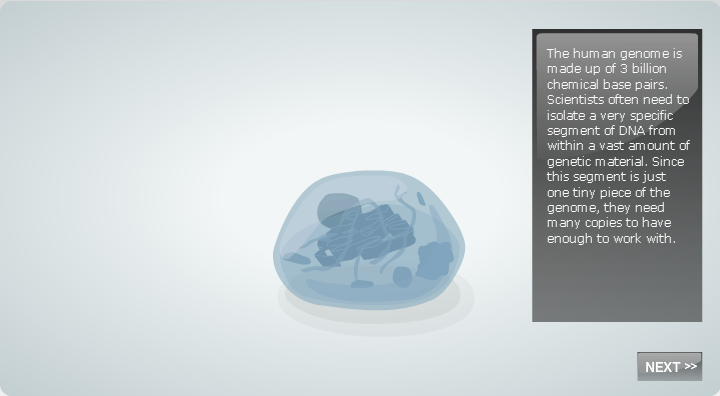
\includegraphics[width=0.8\textwidth]{./img/currentSystems3-1.png}
  \end{center}
\end{figure}
\end{frame}

\begin{frame}
\frametitle{Current Systems [3]}
\begin{figure}
  \begin{center}
    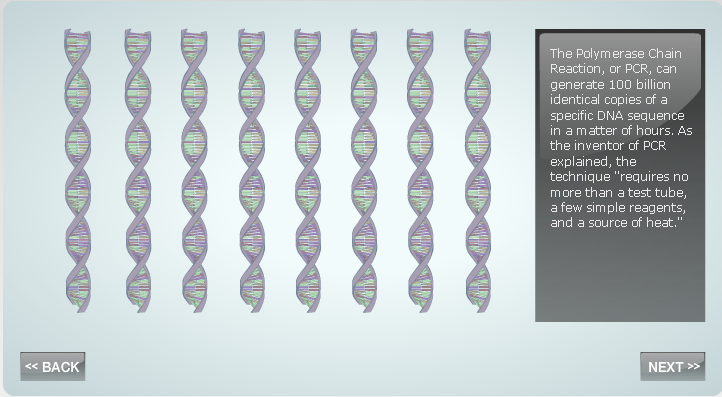
\includegraphics[width=0.8\textwidth]{./img/currentSystems3-2.png}
  \end{center}
\end{figure}
\end{frame}

\begin{frame}
\frametitle{Current Systems [3]}
\begin{figure}
  \begin{center}
    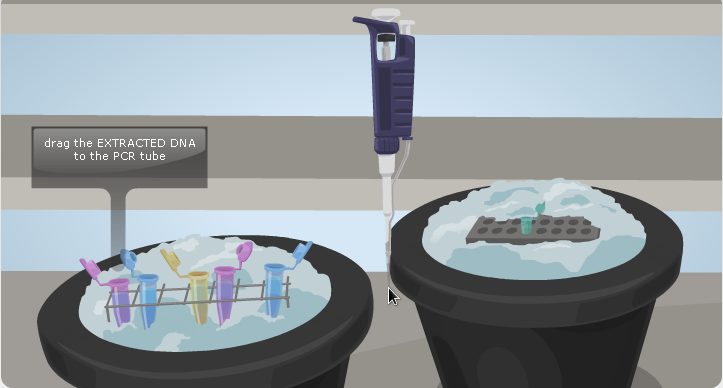
\includegraphics[width=0.8\textwidth]{./img/currentSystems3-4.png}
  \end{center}
\end{figure}
\end{frame}

\begin{frame}
\frametitle{Current Systems [3]}
\begin{figure}
  \begin{center}
    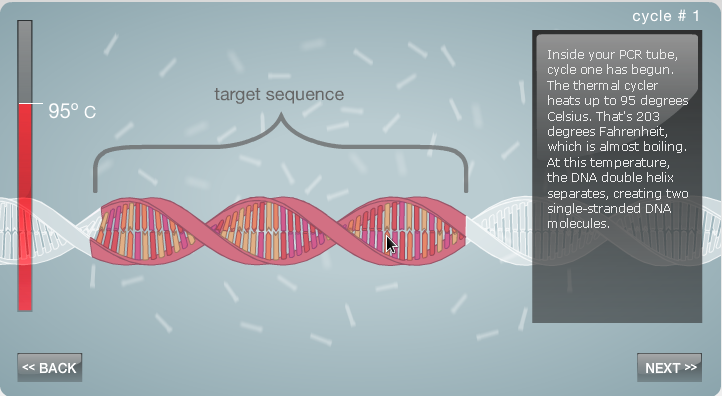
\includegraphics[width=0.8\textwidth]{./img/currentSystems3-5.png}
  \end{center}
\end{figure}
\end{frame}

\begin{frame}
\frametitle{Current Systems [3]}
\begin{figure}
  \begin{center}
    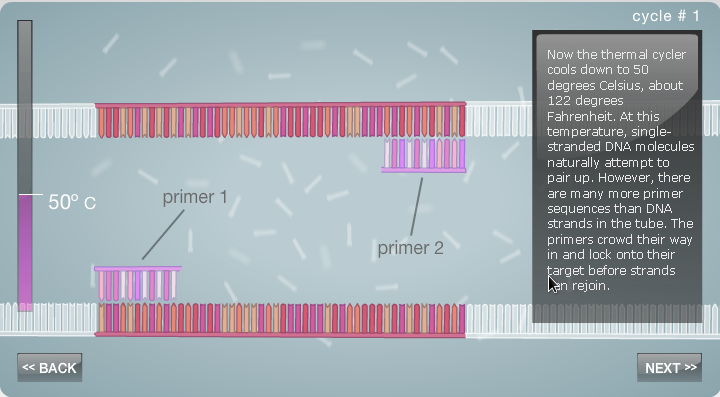
\includegraphics[width=0.8\textwidth]{./img/currentSystems3-6.png}
  \end{center}
\end{figure}
\end{frame}

\begin{frame}
\frametitle{Differences}
\begin{itemize}
\item Focus heavily on Primer Design aspect.
\item Interactivity - allow the user to design their own primers and get
immediate feedback on what they have done right or wrong.
\end{itemize}
\end{frame}


















\section{Evaluation}
   
\begin{frame}
\frametitle{Demonstration Run}
\item Group of people from School of Life Sciences, students and lecturers
\item demoBuild
\item Provided with User Guide
\item No dynamic highlighting or animation
\item Team was on hand
\item Ran for 30 mins, then had roundtable discussion
\item Feedback forms
\end{frame}    


  
\begin{frame}
\frametitle{Demonstration Feedback}
\item Lots of varied discussion - some good, some bad
\item Users tended not to comment on parts that worked
\item Collated results, then decided what needed to be changed
\end{frame}    

\begin{frame}
\frametitle{Demonstration Points}
\item Users felt program was better than paper, and layout was very functional
\item Reverse primers would dissapear - Make sure they were stored and add highlighting
\item Rules were unbreakable in system - Add an override function
\item No graphical copy/paste - add a menu with copy/paste
\item Capitalisation seemed very harsh
\item Temperature bug present in system
\item Couldn't check each primer seperately - implement buttons for this

\end{frame}    




\section{Future Work}
With regards to future work on the project, we feel there are various improvements and tweaks that could be made to the application in order to improve it. These changes can be made in the future, in order to make it a better and more complete teaching tool for the School of Life Sciences.

Also with regards to the feedback (See: Appendix \ref{app:questionnaireResponses}), we will continue to monitor any feedback from the students for any bugs we may need to fix, or any improvements they suggest. Whilst the feedback we recieved has been mostly positive, it has highlighted areas in which the program can be modified and improved.

\subsection{Future Improvements}

Adding a highlighting primer function on the double stranded screen. This feature was never implemented due to the time constraints of the project. However, for the final application it would certainly improve usability for the user. It would also increase familiarity for the user, as they would see the same features implemented over each primer selection screen. \\ \\

Whilst we did not envisage for this to be a problem, thanks to the feedback (See: Section \ref{eval:question}) provided it was clear that a user may try to enter their primer in using capital letters, for whatever reason. Therefore, a function that ensures that if the user enters a sequence of capital letters into a primer box, that it will highlight it on the DNA sequence regardless, should be implemented in the code for the program, to ensure this bug is fixed. \\ \\

It has been noted that the standard resolution of the application begins at 800 x 600, but when the application reaches the animation panel it changes to 1024 x 768. A further improvement to be made therefore would be to fix the inconsistencies in the resolution, making it a standard size throughout usage. \\ \\

We have discussed perhaps implementating a 'hints' system for primer design. This would try to guide the user when they enter an incorrect primer, perhaps suggesting some tips or methods to improve it, especially if it is close to passing the tests. The rules however are already provided for the user to view at their discretion however. \\ \\

One issue that was raised in the questionaire feedback (See: Appendix \ref{app:questionnaireResponses}) was that the animation would not run on a computer located on the Glasgow University campus (They say level 8 - as there isn't many buildings with computers this high we have taken the presumption that they mean a machine in the library). Due to this, we have decided to investigate the portability of the application further, with particular regards to the animation sequence. Whilst we had tested for this beforehand more testing is required to find out the cause of this problem. \\ \\

Another possible improvement to the application would be to remake the application in flash \cite{Flash}. Flash is a global standard platform for static animations, and could possibly bring improvements to the look and feel of the application. \\ \\

The font size in the application is set to a standard size, and cannot be changed. An improvement that has been suggested to the implementation is that we allow the user to change the font size, to allow more accessibility. \\ \\

A bug has been noted in further testing in the dynamic highlighting function. This occurs when a sequence is entered into the box, and due to the combination of the letters two sequences overlap each other, it will only highlight the first sequence on the chosen DNA. The proposed change to the function would highlight both these sequences, in different colours to indicate the difference. \\ \\

Users have commented that the program looks very clinical and simple, keeping to a functional layout. Whilst this is a strong point of the program, it could perhaps be altered slightly with such alterations as images, different colour schemes, diagrams etc. \\ \\














\section{Requirements gathering}
\frame{\titlepage}

\begin{frame}
\frametitle{Requirements gathering - Initial data}
At the first meeting with the clients we were provided a document outlining the requirements for the end product. The aim of the project was described as follows:
\begin{quotation}
To design a PCR-primer design exercise to complement teaching of a
Molecular Methods course to Level 3 Life Sciences Undergraduates. This
exercise will be integrated into a new part of the lab which we are
designing based around diagnosis of HIV using PCR. You will need to
understand the theory behind PCR and primer design in order to achieve
this.
\end{quotation}
\end{frame}    

\begin{frame}
\frametitle{Requirements gathering - System Scope}
\begin{itemize}
\item{The application should be usable in a teaching environment or by people on their home computers.}
\item{It should function as an interactive, step-by-step guide through 
the process of PCR on a DNA strand of the user's choice.}
\item{The system should also provide the user help with completing each 
task by providing relevant rules for each task.}
\item{When the user has completed the required tasks, the system will then show an animation of the PCR reaction taking place.}
\end{itemize}
\end{frame}

\begin{frame}
\frametitle{Requirements gathering - feedback}
Throughout the project, we maintained weekly meetings with our supervisor and the clients, and this allowed us to iteratively improve our design and, later on, the application itself. We received substantial feedback on the User Interface and the primer check handling, which allowed us to make the application more valuable as a teaching tool.
\end{frame}



\section{UI Draft}


\begin{frame}
\frametitle{UI Draft}
\framesubtitle{The User Interface design was developed based on the feedback and
guidelines set by the clients. Four main stages of the UI were separated into five slides.}



\begin{figure}[h]
  \begin{center}
	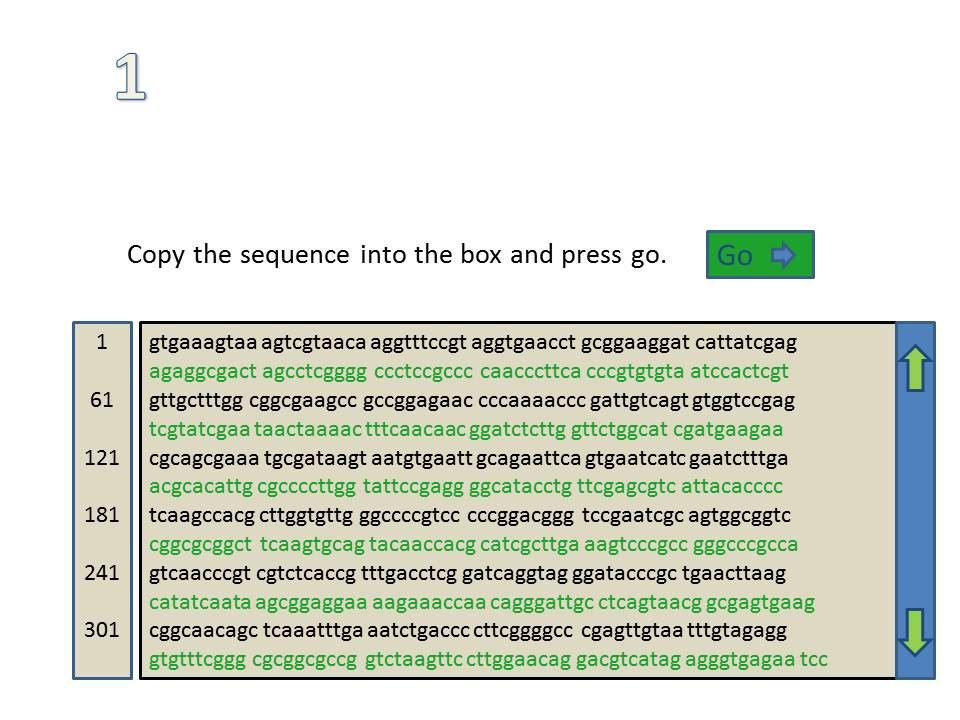
\includegraphics[width=0.8\textwidth]{./img/UiDes/Slide1.JPG}
    \caption{
      \label{fig:UiDes:slide1}
      Initial design, Sequence entry
    }
  \end{center}
\end{figure}
\end{frame}

\begin{frame}

\begin{figure}[h]
  \begin{center}
	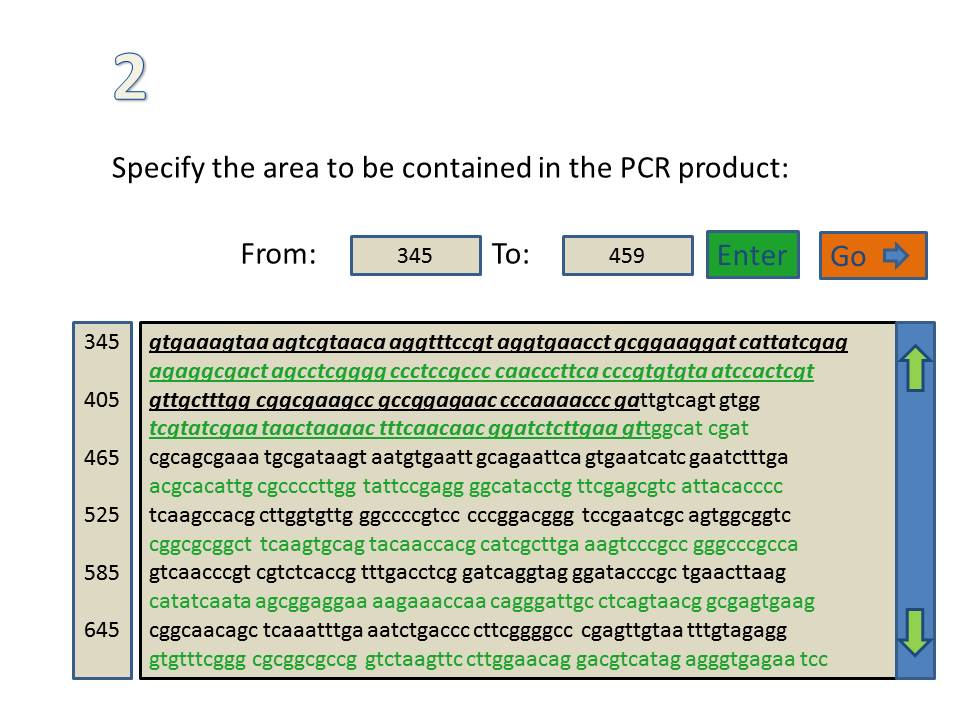
\includegraphics[width=0.8\textwidth]{./img/UiDes/Slide2.JPG}
    \caption{
      \label{fig:UiDes:slide2}
      Initial design,Specification of target area
    }
  \end{center}
\end{figure}

\end{frame}

\begin{frame}

\begin{figure}[h]
  \begin{center}
	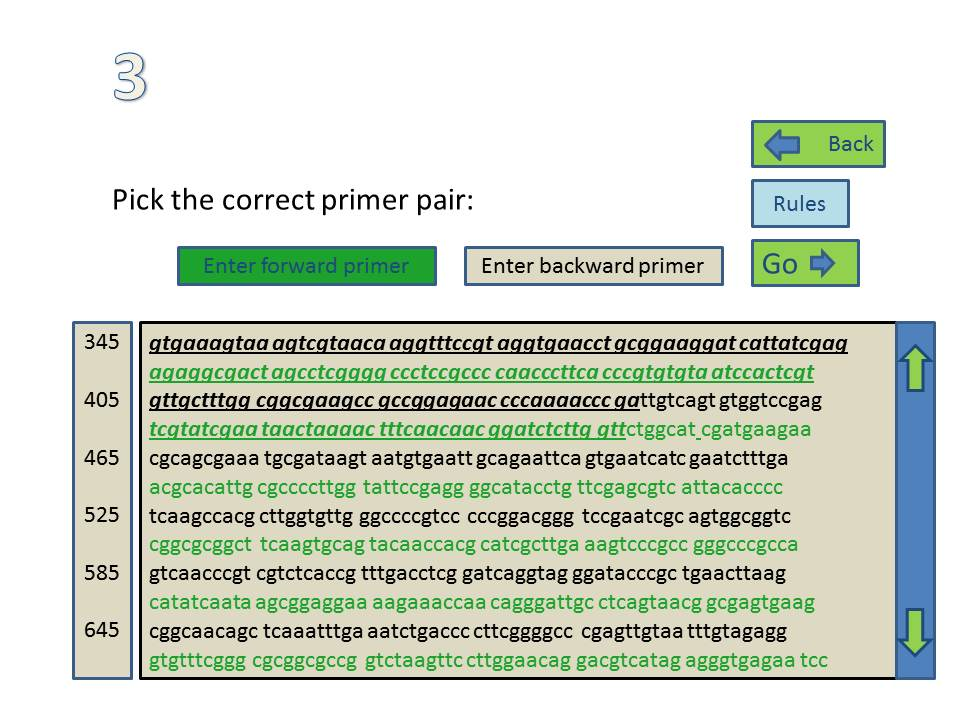
\includegraphics[width=0.8\textwidth]{./img/UiDes/slide3.jpg}
    \caption{
      \label{fig:UiDes:slide3}
      Initial design, Primer selection - initial screen
    }
  \end{center}
\end{figure}

\end{frame}

\begin{frame}

\begin{figure}[h]
  \begin{center}
	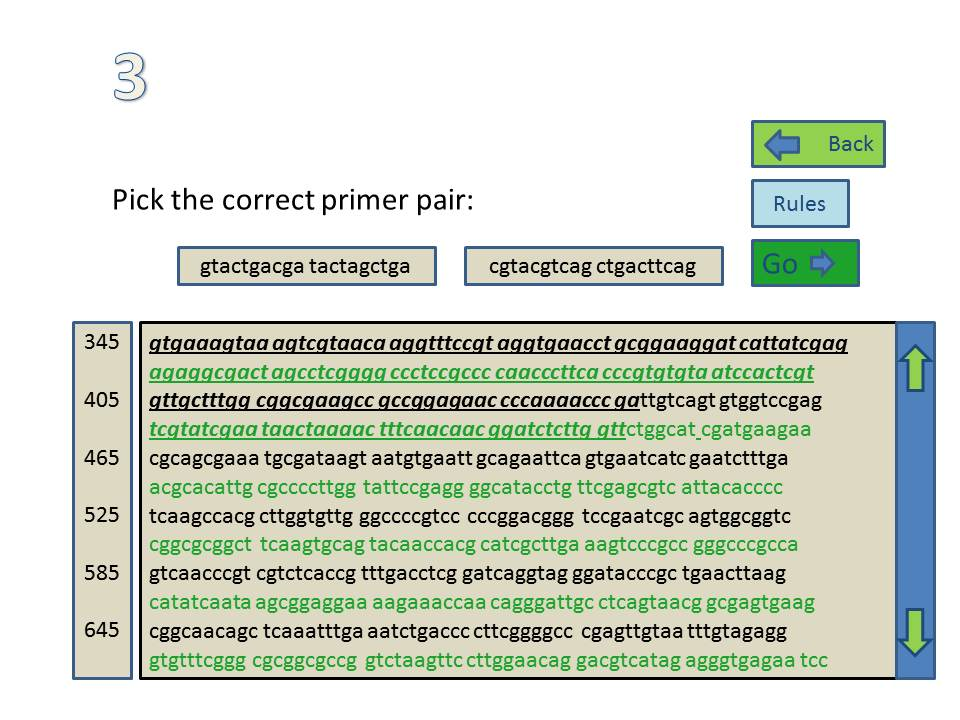
\includegraphics[width=0.8\textwidth]{./img/UiDes/Slide4.JPG}
    \caption{
      \label{fig:UiDes:slide4}
      Initial design, Primer selection - primers entered
    }
  \end{center}
\end{figure}

\end{frame}

\begin{frame}

\begin{figure}[h]
  \begin{center}
	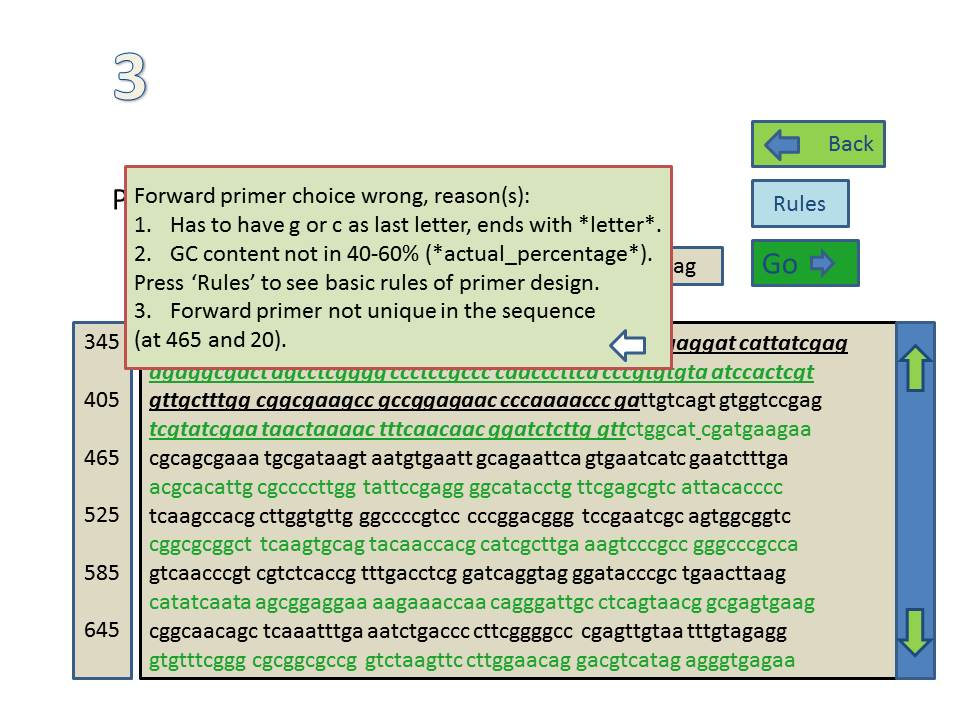
\includegraphics[width=0.8\textwidth]{./img/UiDes/slide5.jpg}
    \caption{
      \label{fig:UiDes:slide5}
      Initial design, Primer selection - error message
    }
  \end{center}
\end{figure}

\end{frame}



\section{Animation}


\begin{frame}
\frametitle{Animation}
The animation was developed based on the sample animations suggested to us by the clients and is split into 7 stages, each with a related explanatory statement at the bottom. It also includes a thermometer and four buttons for animation control.
\end{frame}

\begin{frame}
In the stages 0 and 1, PCR is briefly explained in simple terms as the temperature rises to 72\degree C.
\begin{figure}[h]
  \begin{center}
	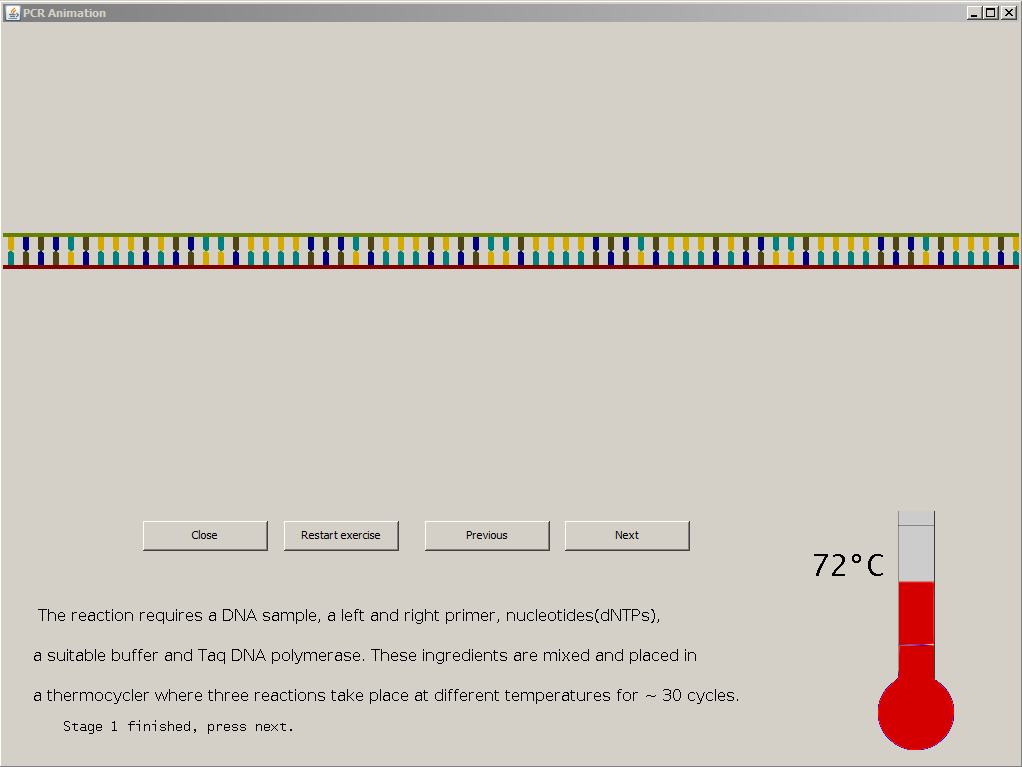
\includegraphics[width=0.7\textwidth]{./img/AnimImpl/Stage1.png}
    \caption{
      \label{fig:AnimImpl:stage1}
      Animation, Stage 1
    }
  \end{center}
\end{figure}
\end{frame}


\begin{frame}
In stage 2, Melting and Annealing, the strands are separated and the primers bind to them, with the temperature level varying accordingly.

\begin{figure}[!t]
  \begin{center}
	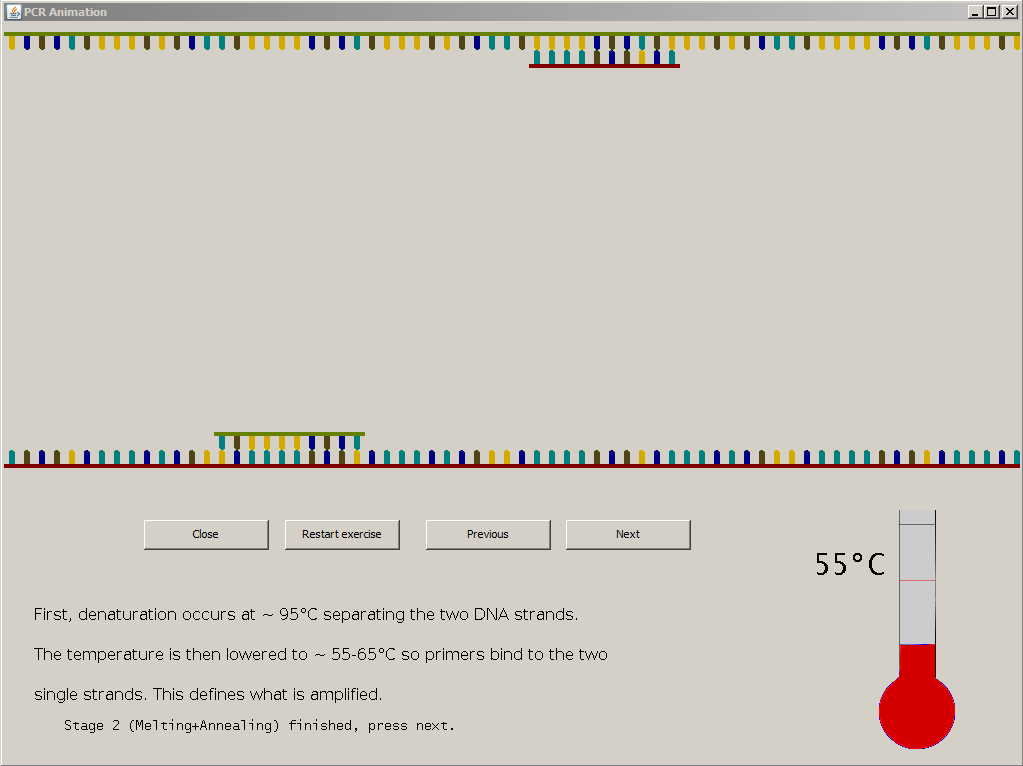
\includegraphics[width=0.7\textwidth]{./img/AnimImpl/Stage2.png}
    \caption{
      \label{fig:AnimImpl:stage2}
      Animation, Stage 2
    }
  \end{center}
\end{figure}
\end{frame}

\begin{frame}
In stage 3, Adding nucleotides, the taq polymerase creates a complementary copy of each strand, with the temperature once again raised to 72\degree C.

\begin{figure}[!t]
  \begin{center}
	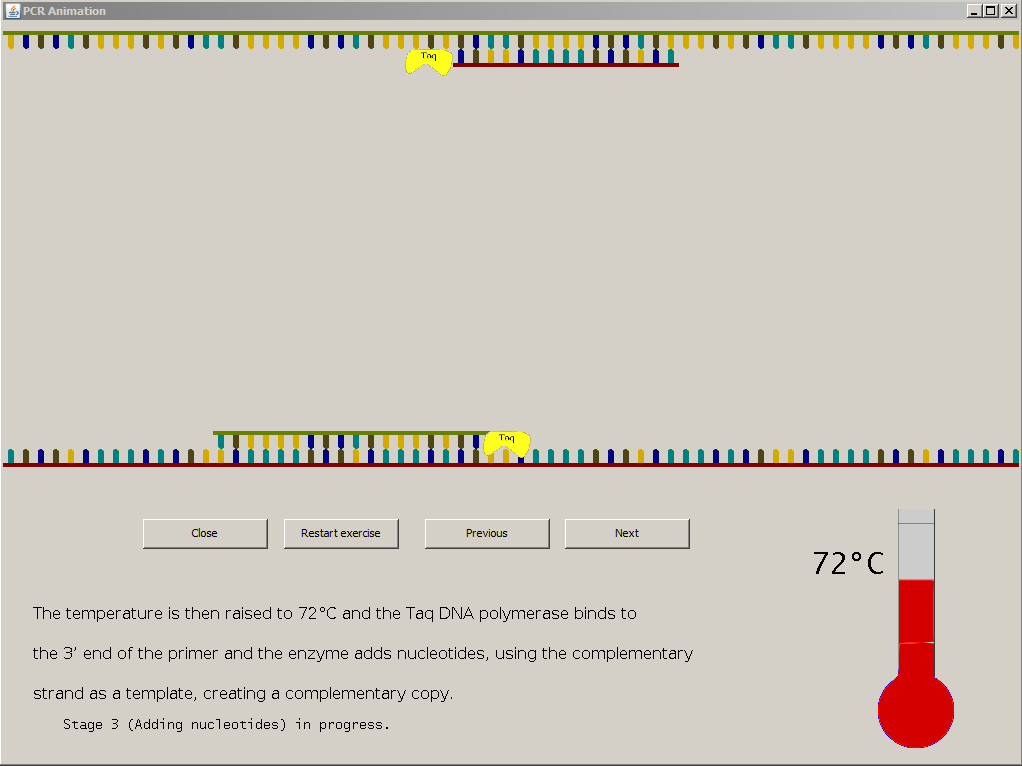
\includegraphics[width=0.7\textwidth]{./img/AnimImpl/Stage3.png}
    \caption{
      \label{fig:AnimImpl:stage3}
      Animation, Stage 3
    }
  \end{center}
\end{figure}
\end{frame}

\begin{frame}

In stages 4 and 5 another cycle of PCR is shown and the required sequence is generated for the first time.

\begin{figure}[!t]
  \begin{center}
	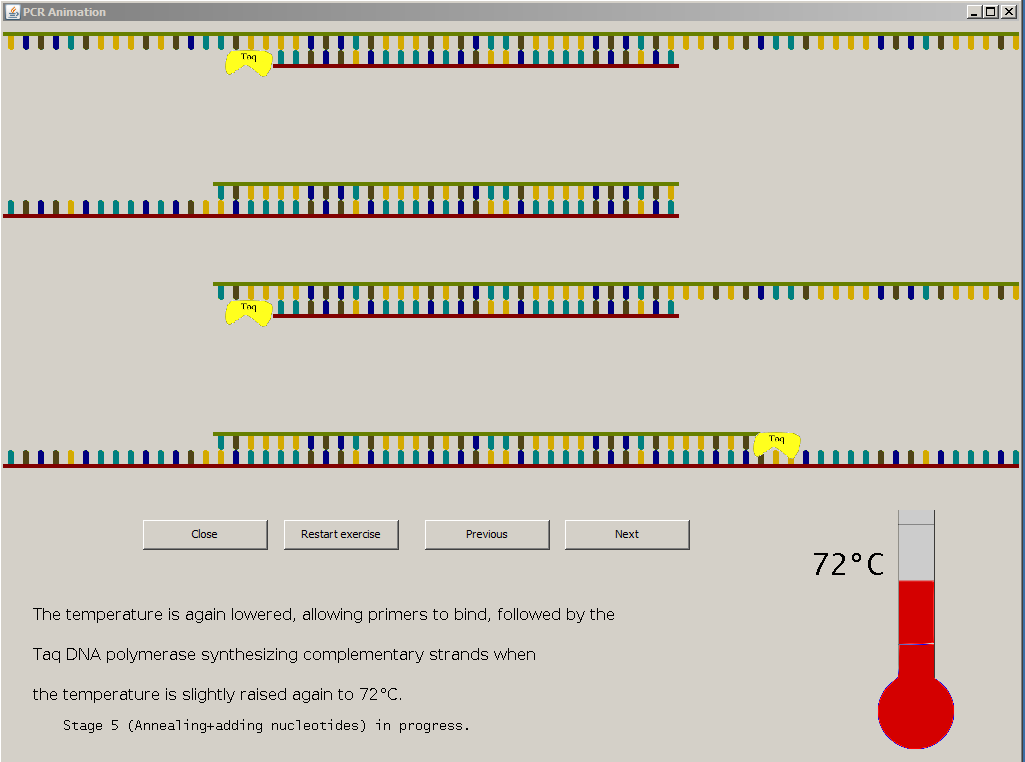
\includegraphics[width=0.7\textwidth]{./img/AnimImpl/Stage5.png}
    \caption{
      \label{fig:AnimImpl:stage5}
      Animation, Stage 5
    }
  \end{center}
\end{figure}
\end{frame}

\begin{frame}
Finally, the last two stages explain how many copies of the target sequence is produced in subsequent cycles and the user is explained that they completed the exercise and thanked for participation.

\begin{figure}[!t]
  \begin{center}
	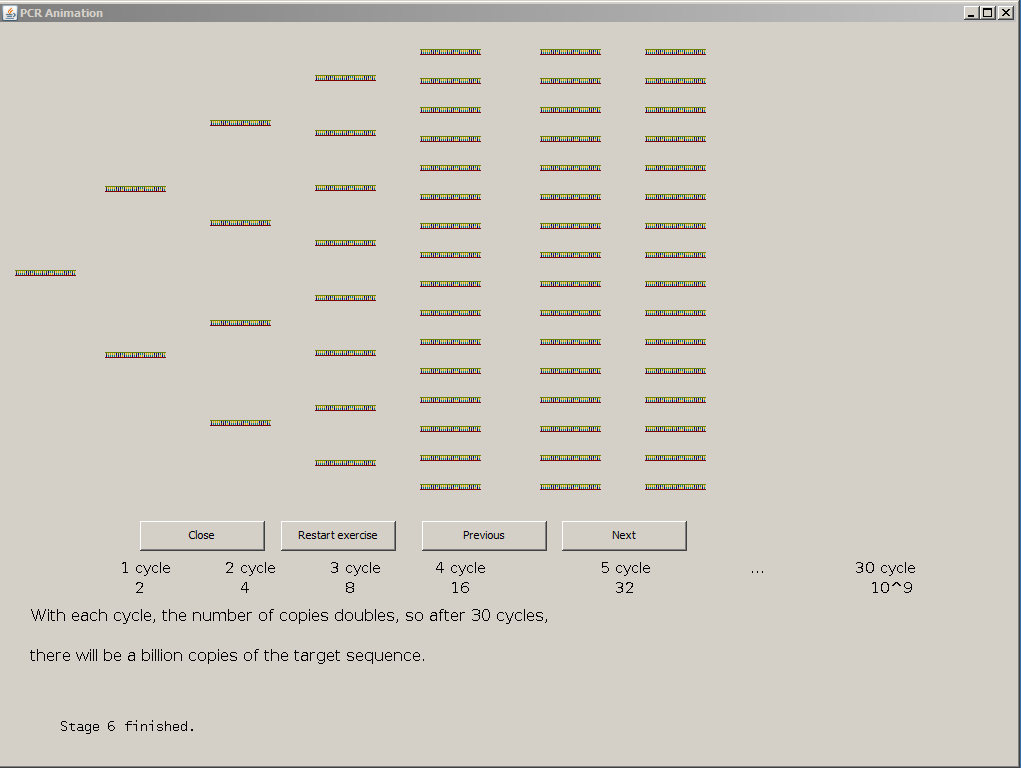
\includegraphics[width=0.7\textwidth]{./img/AnimImpl/Stage6.png}
    \caption{
      \label{fig:AnimImpl:stage6}
      Animation, Stage 6
    }
  \end{center}
\end{figure}
\end{frame}


\end{document}
